\documentclass[a4paper,12pt]{article}
	\usepackage[left=2cm,right=1cm,top=1cm,bottom=1.5cm]{geometry}
	\usepackage[utf8]{inputenc}
	\usepackage[english,russian]{babel}
	\usepackage{graphicx}
	\usepackage{amsmath}
	\usepackage{amssymb}
	\usepackage{cite}
	\usepackage{indentfirst}
	\usepackage{multicol}
	\usepackage{cmap}
	
	\sloppy
	
	\usepackage{geometry}
	\geometry{top=2cm}
	\geometry{bottom=2cm}
	\geometry{left=2.5cm}
	\geometry{right=2.5cm}
	
	\renewcommand{\baselinestretch}{1.5}
	
	\begin{document}
		\renewcommand{\contentsname}{\Large Содержание}
		\renewcommand{\bibname}{\normalfont\Large\bfseries Список литературы}
		
		\begin{titlepage}
			\begin{center}
				Министерство науки и высшего образования Российской Федерации \\
				НАЦИОНАЛЬНЫЙ ИССЛЕДОВАТЕЛЬСКИЙ ЯДЕРНЫЙ УНИВЕРСИТЕТ <<МИФИ>> \\*
				\hrulefill\\
			\end{center}
		
		\begin{center}
			ИНСТИТУТ ЛАЗЕРНЫХ И ПЛАЗМЕННЫХ ТЕХНОЛОГИЙ\\
			КАФЕДРА №31 ПРИКЛАДНАЯ МАТЕМАТИКА
		\end{center}
		\vspace{1cm}
		
		\vspace{2em}
		
		\begin{center}
			\large{Отчет}
			
			по проектной практике на тему:
		\end{center}
		
		\begin{center}
			\large Численное исследование уравнения Минорского
		\end{center}
	
	

\vspace{32em}
		
		\begin{center}
			г. Москва 2024
		\end{center}
	\end{titlepage}

	\newpage
	\section*{Аннотация}
	
	В данной работе провели численное исследование уравнения Минорского,
которое встречается в различных механических и электротехнических задачах, 
где имеется запаздывание и нелинейность. Были реализованы явная и неявная 
схемы Эйлера первого и второго порядка точности соответственно, метод 
подстановки второго порядка и метод Рунге-Кутты четвёртого порядка точности для 
уравнения Минорского. Получены зависимости погрешности от шага разбиения. 
Проведено исследование уравнения при различных параметрах, построили графики 
решения и фазовые плоскости.
Также была проверена сеточная сходимость использованных методов, 
при помощи тестовой задачи.

    \newpage 
	\tableofcontents
	\setcounter{page}{3}

	\newpage
	\section{Постановка задачи}
	Численно исследовать уравнение Минорского.

    Уравенение имеет вид:
    \begin{equation}
    y'' + 2ry' + w^2y + 2qy'(t - 1) = \varepsilon y'^3(t - 1)
	\label{f1}
    \end{equation}
    Здесь r = -1, q = -1, \(\omega = \pi n\). Начальные данные задаются при всех
    \(t \in [-1, 0 ]\). Построить графики решения и фазовые портреты.
	
    \section{Методы решения}
	Для решения поставленной задачи Коши использовались численные методы решения 
	дифференциальных уравенений.

	Первым использованным методом является \textit{явная схема Эйлера} -~метод с самым 
	маленьким порядком точности равным единице.
	Метод вглядит следующим образом.

	Рассмотрим задачу Коши для системы дифференциальных уравнений первого
	порядка:

	\begin{equation}
		\begin{cases}
			x^\prime = f(x, t); \\
			x(t_0) = x_0.
		\end{cases}
		\label{f2}
	\end{equation}

	Переход от $(x_n, y_n)~\text{к}~(x_{n+1}, y_{n+1})$
	производится следующим образом:

	\begin{center}
	$x_{n+1} = x_n + \tau f(x_n, t_n)$
	\end{center}

	Следующей рассматривается \textit{неявная схема Эйлера} -~метод второго порядка.
	Имеет следующий вид для задачи Коши (\ref{f2}), рассмотренной выше:
	
	Переход от $(x_n, y_n)~\text{к}~(x_{n+1}, y_{n+1})$
	производится следующим образом:

	\begin{center}
	$x_{n+1} = x_n + \frac{\tau}{2} (f(x_n, t_n) + f(x_{n+1}, t_{n+1}))$
	\end{center}

	Третий -~метод \textit{Рунге-Кутты} второго порядка точности. 
	Переход осуществялется следующим образом:

	Для начала всчитывается вспомогательный параметр
	
	$x^*_{n+1} = x_n + \tau f(x_n, t_n)$

	После делается шаг интегрирования:

	\begin{center}
	$x_{n+1} = x_n + \frac{\tau}{2} (f(x_n, t_n) + f(x^*_{n+1}, t_{n+1}))$
	\end{center}

	Последним использованным методом -~одним из 
	стандартных численных методов решения дифференциальных уравнений, 
	включая уравнения с запаздыванием, явлется классический метод \textit{Рунге-Кутты} 
	чевёртого порядка. Метод выглядит следующим образом.
	Для ананлогичной задачи Коши (\ref{f2}):

	Переход от $(x_n, y_n)~\text{к}~(x_{n+1}, y_{n+1})$ 
	начинается с вычисления вспомогательных параметров:\\
	$k_1 = f(x_n, t_n)$\\
	$k_2 = f(x_n + 0.5 k_1, t_n + 0.5 \tau)$\\
	$k_3 = f(x_n + 0.5 k_2, t_n + 0.5 \tau)$\\
	$k_4 = f(x_n + k_3, t_n + \tau)$\\

	После последовательного вычисления $k_1, k_2, k_3, k_4$ 
	делается шаг интегрирования:

	\begin{center}
		$x_{n+1} = x_n + \frac{\tau}{6}(k_1 + 2k_2 + 2k_3 + k_4)$
	\end{center}

	Таким образом, один шаг требует четырёхкратного перевычисления правой части, 
	что и даёт этому методу четвёртый порядок.

	\section{Проверка точности и сеточной сходимости}
	Для проверки точности реализации использованных методов решим уравнение 
	с запаздыванием, которое имеет известное точное решение. 
	Рассмотрим следующую тестовую задачу:

	\begin{equation}
		x'(t) = - \alpha x(t-1) (1 + x(t)),~\alpha \neq 0
	\end{equation}

	Для начального условия $t_0 = 0$ и начальной функции $\varphi (t) = t$, 
	$t\in [-1,0]$ точное решение задачи Коши на отрезке [0, 1] имеет следующий вид:
	\begin{equation}
		x(t) = \exp(~\frac{\alpha}{2}({(t-1)}^2-1))-1,\:t \in [0, 1]
	\end{equation}

	График искомой функции представлен на рисунке~\ref{fig:fig15}

	\begin{figure}[ht!]
		\begin{center}
		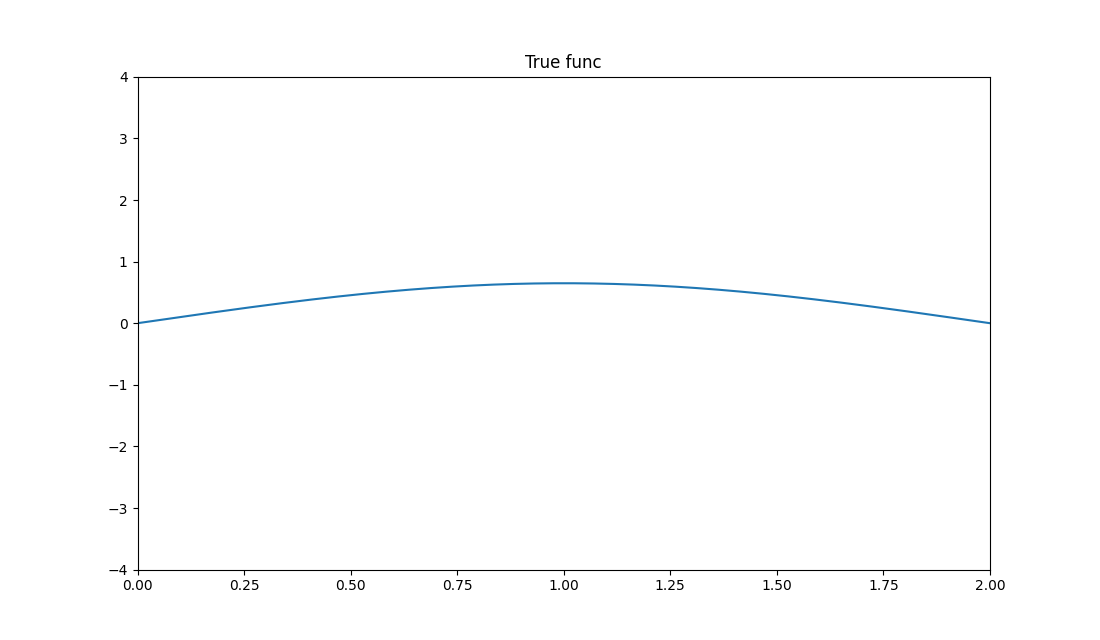
\includegraphics[scale=0.43]{figures/true_1.png}
		\end{center}
		\vspace*{-8mm}
		\caption{График искомой функции}\label{fig:fig15}
  	\end{figure}


	Графики, полученные всеми четырьмя методами представлены на \textit{рисунке}~\ref{fig:fig1}.

	\begin{figure}[ht!]
		\begin{center}
		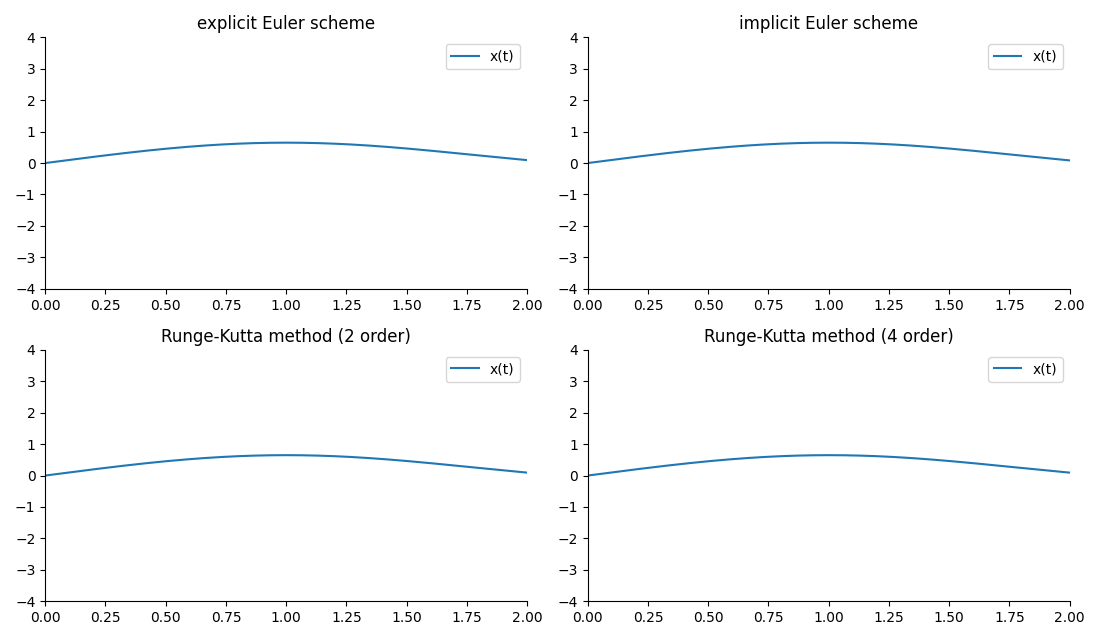
\includegraphics[scale=0.43]{figures/test_1.png}
		\end{center}
		\vspace*{-8mm}
		\caption{Графики функции}\label{fig:fig1}
  	\end{figure}

  	На графиках также указана максимальная погрешность для каждого 
	из методов, и видно, что она не првышает $10^{-5}$.

  	Далее проверили сеточную сходимость методов. Для этого был 
	написан алгоритм, вычисляющий погрешность построения графика 
	искомой функции на данном шаге $\tau$. Зависимость натурального 
	логарифма погрешности от натурального логарифма шага покзана на 
	\textit{рисунке}~\ref{fig:fig2}.

	\begin{figure}[ht!]
		\begin{center}
		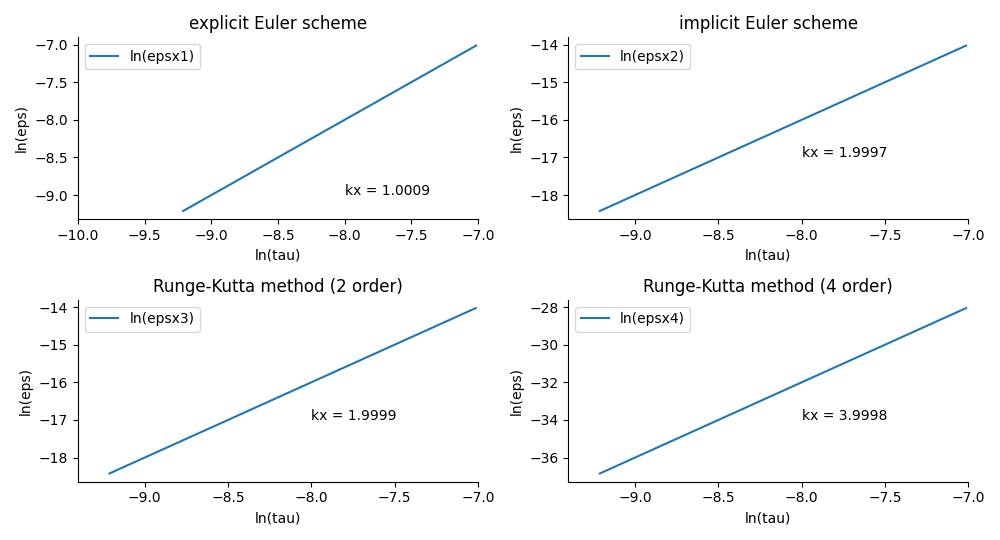
\includegraphics[scale=0.43]{figures/test_2.png}
		\end{center}
		\vspace*{-8mm}
		\caption{График функции и зависимость погрешности от шага $\tau$}\label{fig:fig2}
  	\end{figure}

	Из данных, представленных на графиках, следует, написанные реализации всех 
	четырёх методов соответстуют указанным порядкам точности.

	\section{Решение и исследование уравнения Минорского}
	\subsection{Построение решения}
	Для построения решения уравнения Минорского успользуем все 
	рассмотренные в разделе 2 методы. В качестве начальных условий 
	соответствующей задачи Коши будем брать следующие:	
	$y_0 = y'_0(t-1) = y'_0(t) = 0$;

	Решение уравнения Минорского (\ref{f1}), так как оно нелинейное (второго порядка) 
	сводится к системе линейных уравнений путём замены первой производной функции:
	
	\begin{equation}
		\begin{cases}
			y^\prime = z(t); \\
			z^\prime = \varepsilon z^3(t-1) - 2rz - \omega^2 y - 2q z(t-1);\\
		\end{cases}
		\label{cs1}
	\end{equation}

	В таком случае из-за запаздывания аргумента нужно рассматривать ещё 
	и начальные значения для производной функции $y' = z$ на отрезке $[-1, 0]$.
	Функция $z(t)$ должна являться гладкой на рассматриваемом отрезке доопределния,
	поэтому будем задавать её определённой функцией.

	В качестве шага $\tau$ возьмём 0.00001, а отрезок исследования $[0, 2]$. 
	Для начала рассмотрим уравнение Минорского при значении $n = 3$, а функцию 
	$z(t-1) = t$. 
	Ниже представлены графики функций $y(t)$, $z(t)$ и фазовые портреты $y(z)$
	(см. рисунок~\ref{fig:fig3})

	\begin{figure}[ht!]
		\begin{center}
		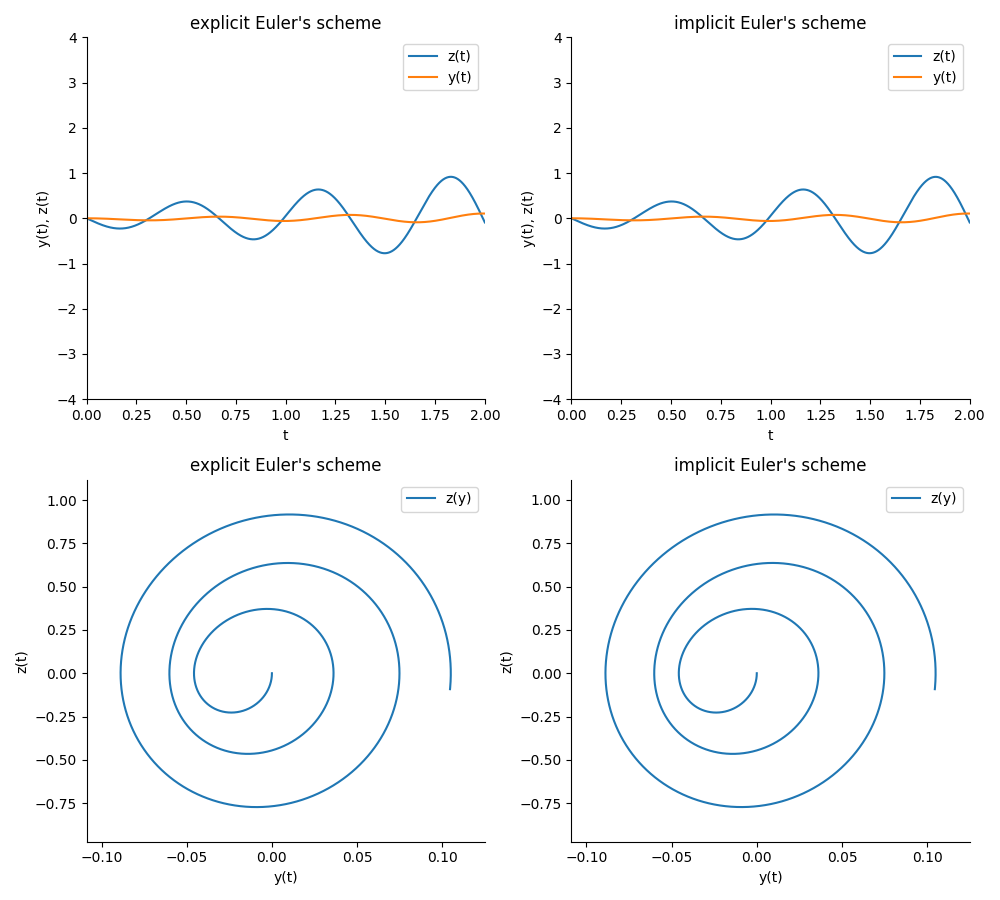
\includegraphics[scale=0.38]{figures/Figure_worked2.png}
		\end{center}
		\vspace*{-8mm}
		\caption{График функции и зависимость погрешности от шага $\tau$ для первых двух методов}\label{fig:fig3}
  	\end{figure}

	  \begin{figure}[ht!]
		\begin{center}
		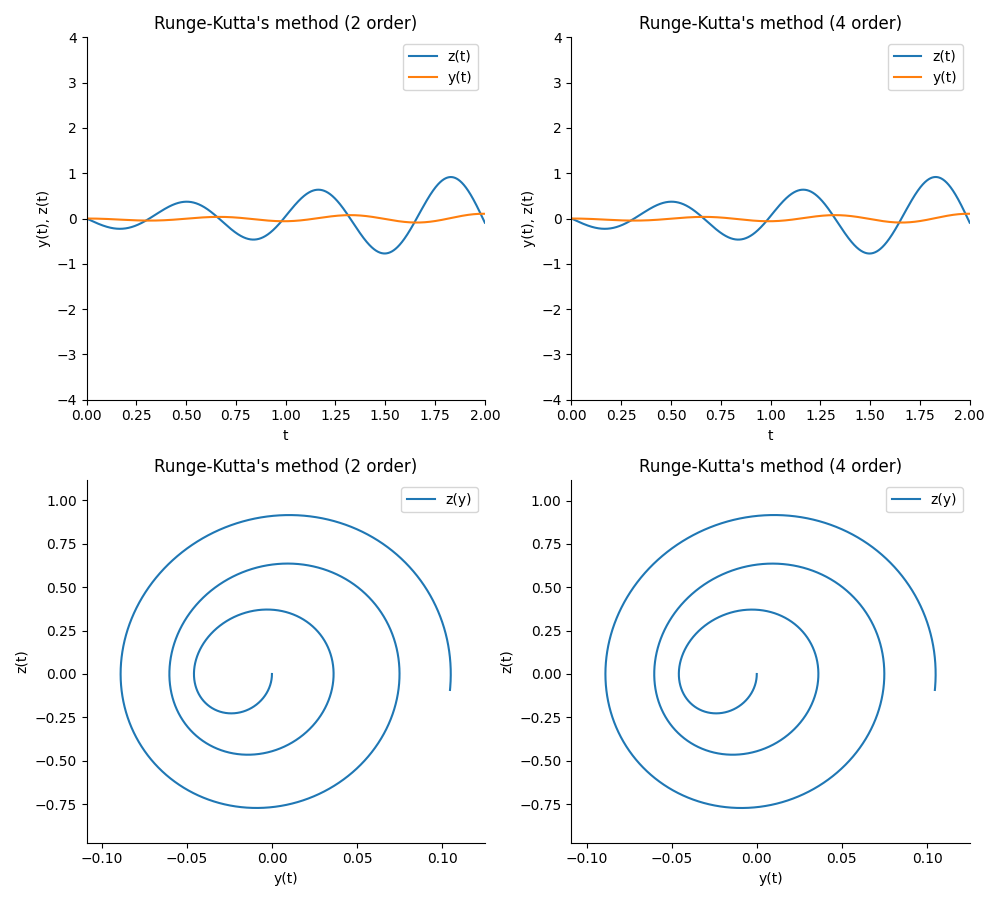
\includegraphics[scale=0.38]{figures/Figure_worked3.png}
		\end{center}
		\vspace*{-8mm}
		\caption{График функции и зависимость погрешности от шага $\tau$ для вторых двух методов}\label{fig:fig4}
  	\end{figure}

	Нетрудно заметить, что производная функции ведёт себя как периодическая 
	функция с постепенно увеличивающейся амплитудой (cм. рис.~\ref{fig:fig3} и~\ref{fig:fig4}).

	\newpage
	\subsection{Анализ поведения функции в зависимости от параметров}
	Рассмотрим, как именно влияет на вид функции доопределение 
	$\varphi(t-1)$.

	\begin{figure}[ht!]
		\begin{center}
		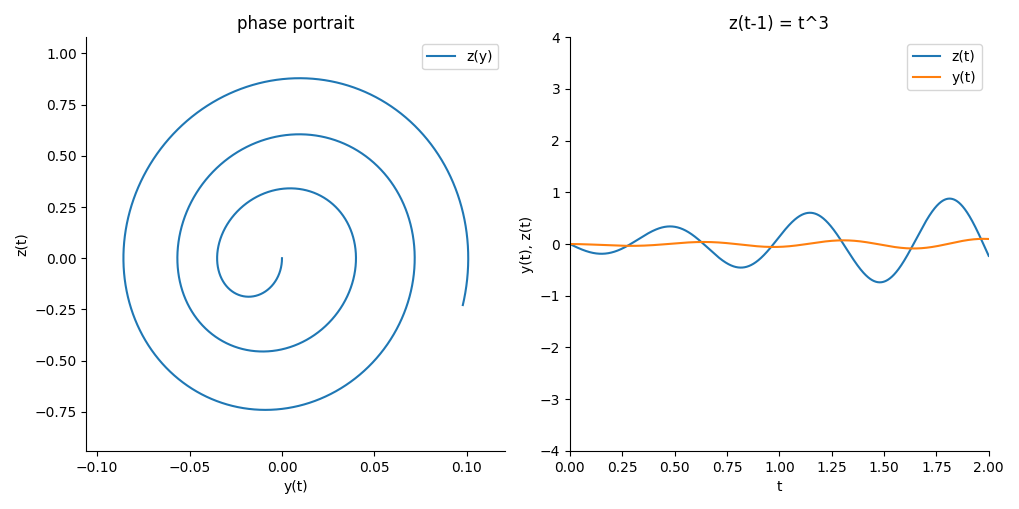
\includegraphics[scale=0.65]{figures/fnc1.png}
		\end{center}
		\vspace*{-8mm}
		\caption{Вид функции при $\varphi(t-1) = t^3$}\label{fig:fig6}
  	\end{figure}

	\begin{figure}[ht!]
		\begin{center}
		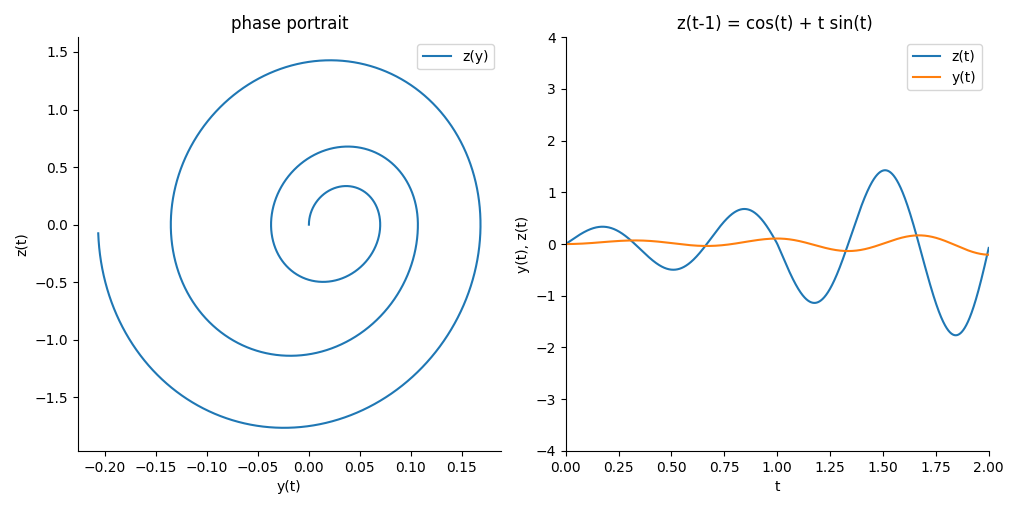
\includegraphics[scale=0.65]{figures/fnc2.png}
		\end{center}
		\vspace*{-8mm}
		\caption{Вид функции при $\varphi(t-1) = \cos(t)+t\sin(t)$}\label{fig:fig7}
  	\end{figure}

	\begin{figure}[ht!]
		\begin{center}
		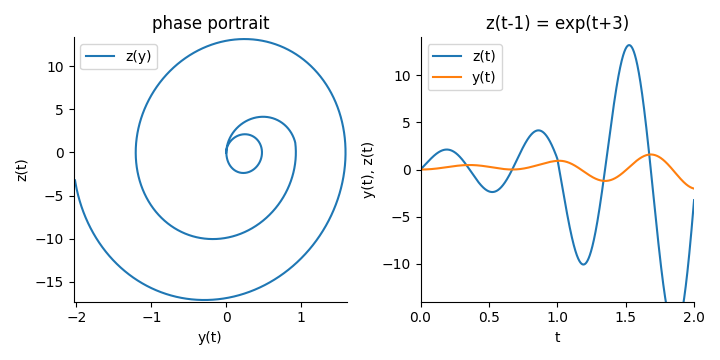
\includegraphics[scale=0.65]{figures/fnc3.png}
		\end{center}
		\vspace*{-8mm}
		\caption{Вид функции при $\varphi(t-1) = \exp(t+3)$}\label{fig:fig8}
  	\end{figure}

	На рисунках~\ref{fig:fig6} -~\ref{fig:fig8} показано, что изменение $\varphi(t-1)$ не влияет на общий 
	вид функции $y(t)$, но заметны различия в характере и скорости роста.

	Теперь рассмотрим поведение функций при изменении параметра n. Для удобства 
	будем рассматривать только метод Рунге-Кутты четвёртого порядка (см. рисунок~\ref{fig:fig5}).

	\begin{figure}[ht!]
		\begin{center}
		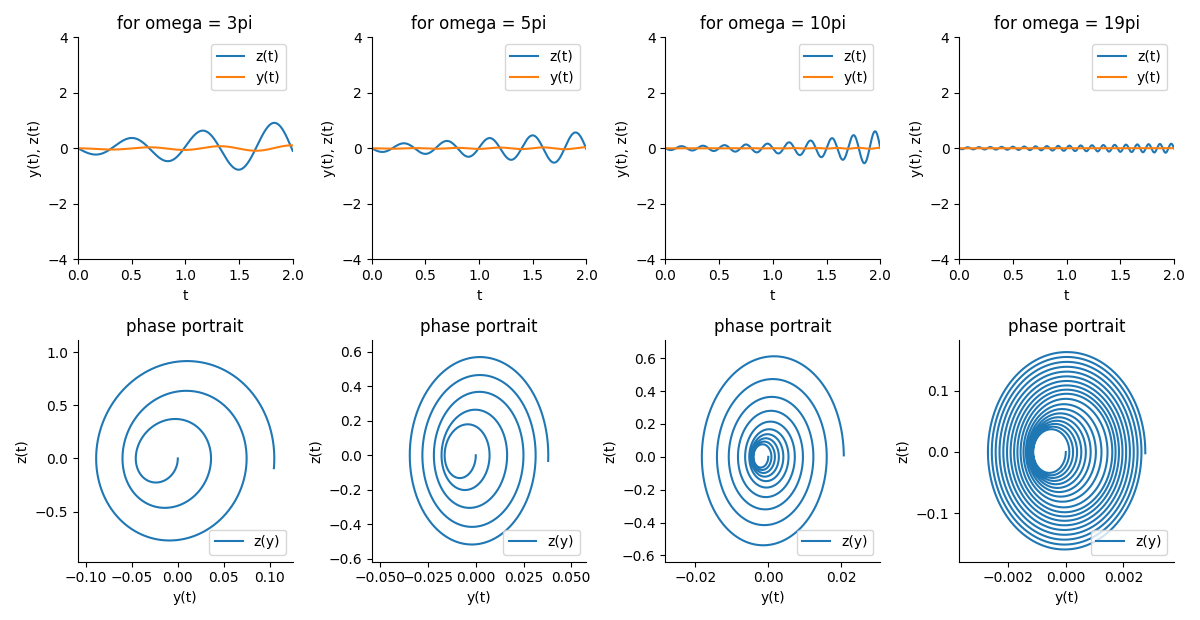
\includegraphics[scale=0.5]{figures/Figure_runge1.png}
		\end{center}
		\vspace*{-8mm}
		\caption{Зависимость функции от параметра n}\label{fig:fig5}
  	\end{figure}

	Для более наглядного и подробного анализа построили трёхмерные фазовые 
	портреты системе координат $t, y(t), z(t)$.

	\begin{figure}[ht!]
		\begin{center}
		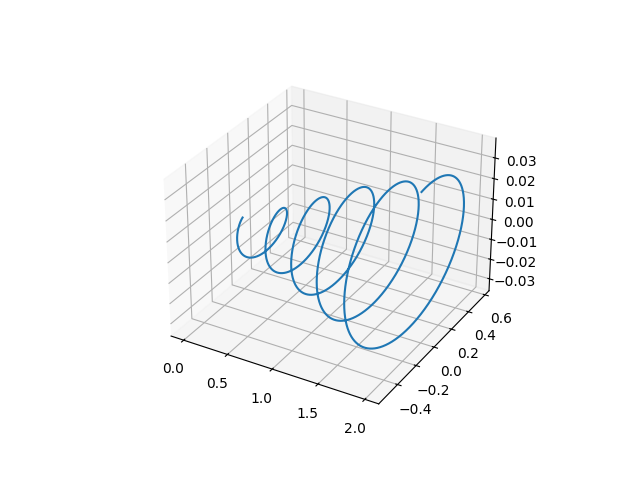
\includegraphics[scale=0.5]{figures/3d_1.png}
		\end{center}
		\vspace*{-8mm}
		\caption{Вид функции $y(z, t)$ при $n = 5$}\label{fig:fig9}
  	\end{figure}

	  \begin{figure}[ht!]
		\begin{center}
		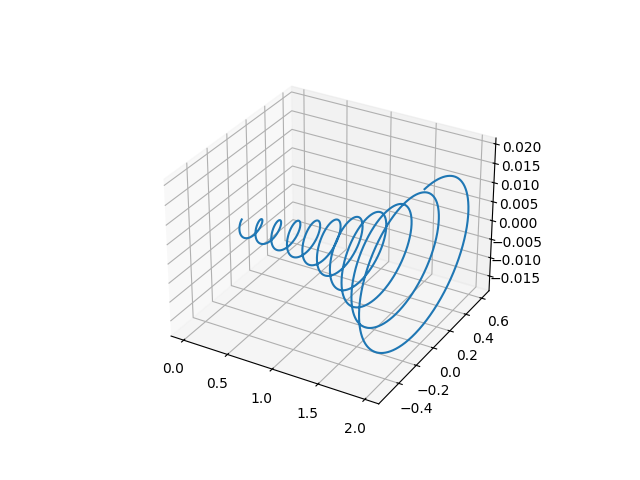
\includegraphics[scale=0.5]{figures/3d_2.png}
		\end{center}
		\vspace*{-8mm}
		\caption{Вид функции $y(z, t)$ при $n = 10$}\label{fig:fig10}
  	\end{figure}

	\begin{figure}[ht!]
		\begin{center}
		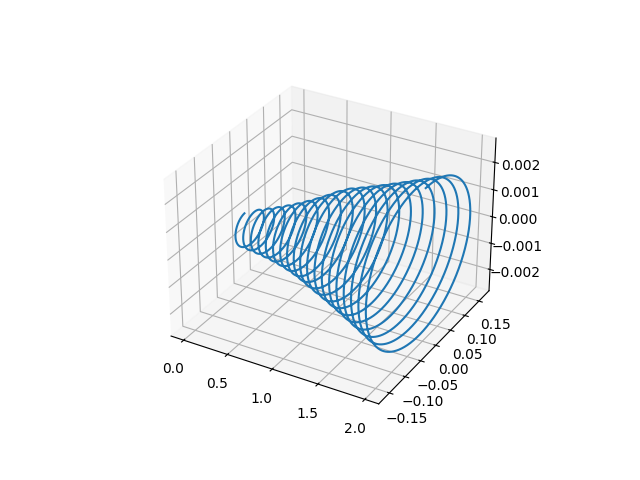
\includegraphics[scale=0.5]{figures/3d_3.png}
		\end{center}
		\vspace*{-8mm}
		\caption{Вид функции $y(z, t)$ при $n = 19$}\label{fig:fig11}
  	\end{figure}

	\newpage
	Таким образом, можно сказать, что период данной функции 
	обратно пропорционально зависит от $\omega$ и от самого параметра n.

	Однако при приближении $|n|$ к единице, вид уравнения начинает 
	становиться неустойчивым (см. рисунок~\ref{fig:fig12}).

	\begin{figure}[ht!]
		\begin{center}
		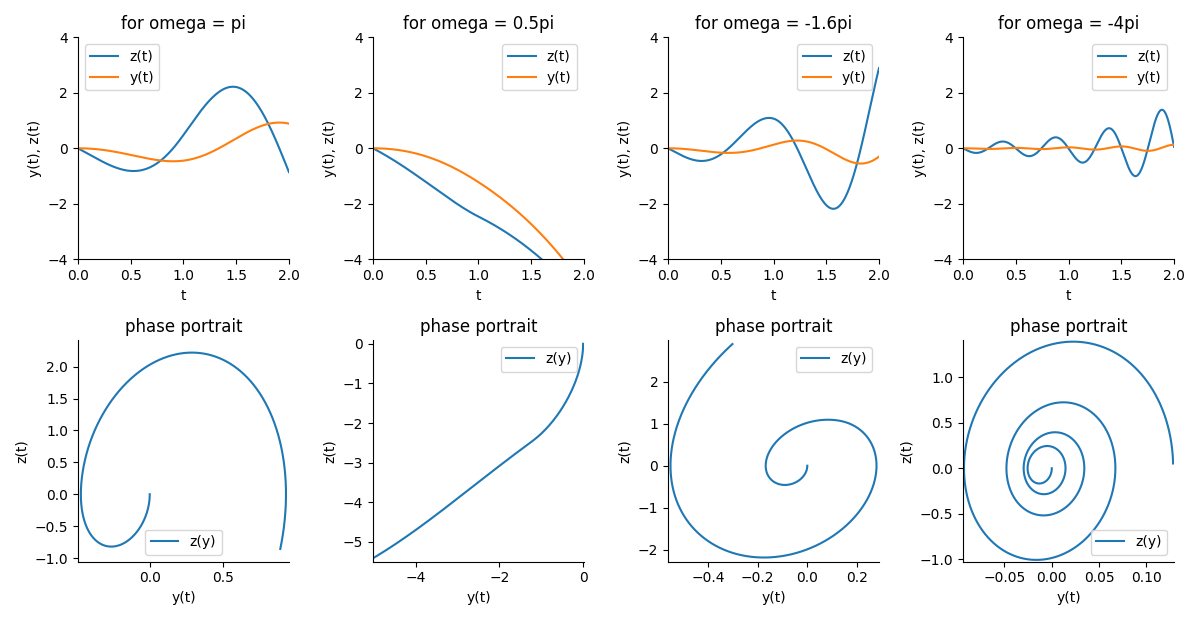
\includegraphics[scale=0.5]{figures/omeg1.png}
		\end{center}
		\vspace*{-8mm}
		\caption{Вид функции при $n\sim0$}\label{fig:fig12}
  	\end{figure}

	Теперь исследуем зависимость от $\varepsilon$. Данный параметр очень 
	мал, $\varepsilon \ll 1$. Рассмотрим поведение 
	функции при соответствующих значениях (см. рисунок~\ref{fig:fig13}).

	\begin{figure}[ht!]
		\begin{center}
		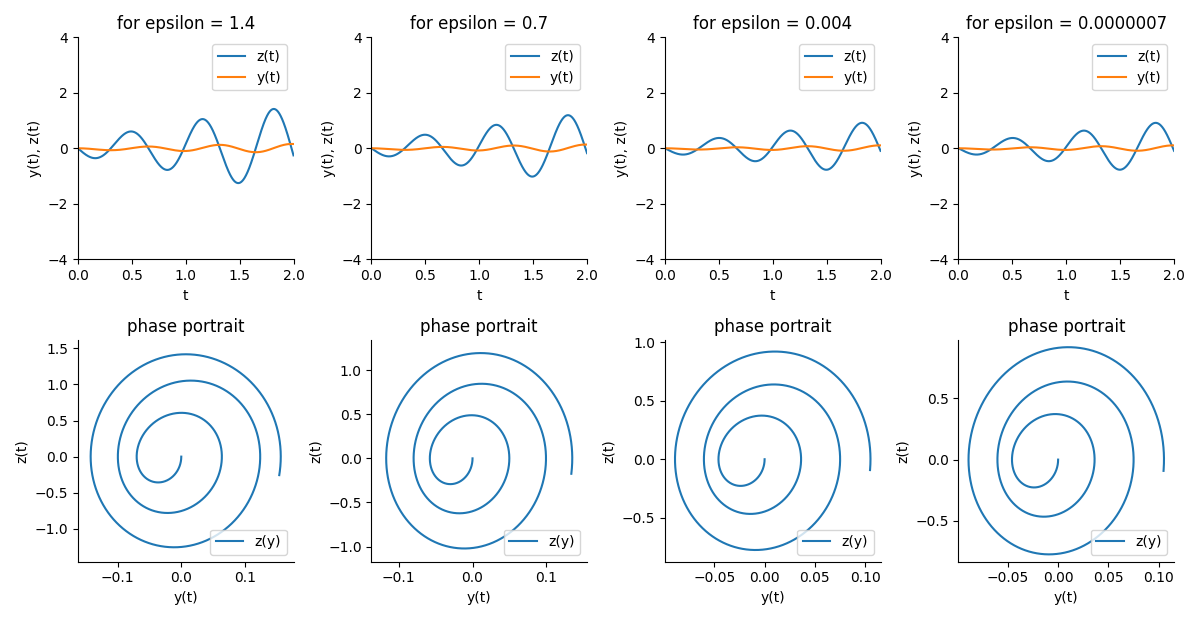
\includegraphics[scale=0.48]{figures/eps1.png}
		\end{center}
		\vspace*{-8mm}
		\caption{Вид функции при малых значениях $\varepsilon$}\label{fig:fig13}
  	\end{figure}

	Стоить отметить, что вид практически не изменяется, идёт небольшое уменьшение амплитуды.
	Однако если пробовать увеличивать $\varepsilon$ до значений, больших единицы, 
	то функция становится неустойчивой (см. рисунок~\ref{fig:fig14}).

	\begin{figure}[ht!]
		\begin{center}
		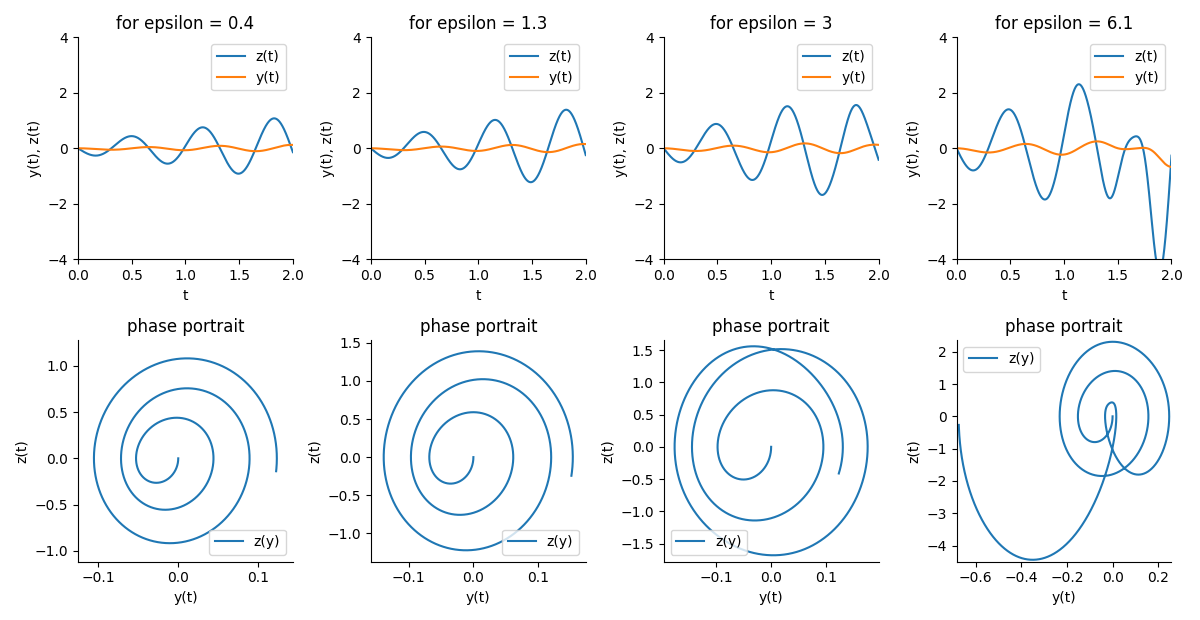
\includegraphics[scale=0.48]{figures/eps2.png}
		\end{center}
		\vspace*{-8mm}
		\caption{Вид функции при больших значениях $\varepsilon$}\label{fig:fig14}
  	\end{figure}

	\section{Заключение}
	В результате выполнения работы по численному исследованию уравнения Минорского 
	были рассмотрены и также исследованы численные методы решения дифференциальных, 
	нелинейных уравнений с запаздыванием. Была написана реализация четырёх таких методов 
	с различными порядками точности и проведена их проверка при помощи тестовой задачи. 
	При использовании рассмотренных методов было численно исследовано уравнение 
	Минорского, для которого были получены графики при различных значениях 
	управляющих параметров. Для более подробного исследования были построены 
	фазовые портреты, показывающие зависимость искомой функции от её производной.


	\newpage
	
	\begin{thebibliography}{w:40}
		
		\bibitem{label1} Рябенький В.С. ``Введение в вычислительную 
		математику''. -~Москва. -~2008.
		\bibitem{label2} Федоренко Р.П. ``Введение в вычислительную физику 
		(2-е издание)''. -~Москва. -~2008.
		\bibitem{label3} Бахвалов Н. С., Жидков Н. П., Кобельков Г М
		``Численные методы''. -~Москва. -~2020.
		\bibitem{label4} Калиткин Н.Н., Корякин П. В. ``Численные методы''. 
		-~Москва. -~2013.
		\bibitem{label5} Петров И. Б. ``Лекции по вычислительной математике. 
		Учебное пособие''. -~Москва. -~2009.
		
	\end{thebibliography}
	
	\end{document}